%% ============================================================================
%%  VLA Robot Learning — Project Report
%%  Author : Sara Aly
%%  Engine : XeLaTeX  (compile with: xelatex REPORT.tex, or python generate_report.py --tex)
%% ============================================================================
\documentclass[12pt, a4paper]{article}

%% ── Encoding & fonts (XeLaTeX) ───────────────────────────────────────────────
\usepackage{fontspec}
\setmainfont{Helvetica Neue}
\setmonofont[Scale=0.88]{Menlo}

%% ── Page layout ──────────────────────────────────────────────────────────────
\usepackage[margin=1in, top=1.2in, bottom=1.2in]{geometry}
\usepackage{setspace}
\onehalfspacing

%% ── Core utilities ───────────────────────────────────────────────────────────
\usepackage{graphicx}
\usepackage{amsmath, amssymb}
\usepackage{microtype}
\usepackage{enumitem}
\usepackage{xcolor}
\usepackage{booktabs}
\usepackage{longtable}
\usepackage{array}
\usepackage{multirow}
\usepackage{caption}
\usepackage{subcaption}

%% ── Colours ──────────────────────────────────────────────────────────────────
\definecolor{NavyBlue}{HTML}{1D4ED8}
\definecolor{LightBlue}{HTML}{DBEAFE}
\definecolor{CodeBg}{HTML}{F8F9FA}
\definecolor{BorderGray}{HTML}{D1D5DB}
\definecolor{TextGray}{HTML}{6B7280}
\definecolor{AlertRed}{HTML}{DC2626}
\definecolor{SuccessGreen}{HTML}{16A34A}
\definecolor{TitleBlue}{HTML}{1E3A5F}
\definecolor{AccentOrange}{HTML}{EA580C}
%% Diagram palette (shared with architecture_diagram.tex)
\definecolor{DarkGreen}{HTML}{15803D}
\definecolor{DimGray}{HTML}{6B7280}

%% ── Section headings ─────────────────────────────────────────────────────────
\usepackage{titlesec}
\titleformat{\section}[block]
  {\Large\bfseries\color{TitleBlue}}{\thesection}{1em}{}
  [\vspace{-4pt}\color{NavyBlue}\rule{\linewidth}{1.2pt}\vspace{4pt}]
\titleformat{\subsection}[block]
  {\large\bfseries\color{TitleBlue}}{\thesubsection}{1em}{}
\titleformat{\subsubsection}[block]
  {\normalsize\bfseries}{\thesubsubsection}{1em}{}

%% ── Header / footer ──────────────────────────────────────────────────────────
\usepackage{fancyhdr}
\pagestyle{fancy}
\fancyhf{}
\fancyhead[L]{\small\textbf{\color{TitleBlue}VLA Robot Learning}}
\fancyhead[R]{\small\color{TextGray}Sara Aly \textbullet{} CSUN}
\fancyfoot[C]{\small\thepage}
\fancyfoot[R]{\small\color{TextGray}Updated: \today}
\renewcommand{\headrulewidth}{0.5pt}
\renewcommand{\footrulewidth}{0.3pt}

%% ── Hyperlinks ───────────────────────────────────────────────────────────────
\usepackage{hyperref}
\hypersetup{
  colorlinks = true,
  linkcolor  = NavyBlue,
  urlcolor   = NavyBlue,
  citecolor  = NavyBlue,
  pdftitle   = {VLA Robot Learning — Project Report},
  pdfauthor  = {Sara Aly, Connor Juman},
  pdfsubject = {Vision-Language-Action Model with RL Feedback},
}

%% ── Code listings ────────────────────────────────────────────────────────────
\usepackage{listings}
\lstdefinestyle{Python}{
  language        = Python,
  basicstyle      = \ttfamily\small,
  keywordstyle    = \color{NavyBlue}\bfseries,
  commentstyle    = \color{TextGray}\itshape,
  stringstyle     = \color{AccentOrange},
  backgroundcolor = \color{CodeBg},
  frame           = single,
  rulecolor       = \color{BorderGray},
  numbers         = left,
  numberstyle     = \tiny\color{TextGray},
  stepnumber      = 1,
  breaklines      = true,
  showstringspaces= false,
  tabsize         = 4,
  xleftmargin     = 18pt,
  framexleftmargin= 14pt,
  aboveskip       = 8pt,
  belowskip       = 8pt,
}
\lstdefinestyle{Bash}{
  language        = bash,
  basicstyle      = \ttfamily\small,
  keywordstyle    = \color{NavyBlue}\bfseries,
  backgroundcolor = \color{CodeBg},
  frame           = single,
  rulecolor       = \color{BorderGray},
  breaklines      = true,
  showstringspaces= false,
  xleftmargin     = 10pt,
  aboveskip       = 6pt,
  belowskip       = 6pt,
}
\lstdefinestyle{Diagram}{
  basicstyle      = \ttfamily\scriptsize,
  backgroundcolor = \color{CodeBg},
  frame           = single,
  rulecolor       = \color{BorderGray},
  breaklines      = true,
  breakatwhitespace = false,
  postbreak       = \mbox{\textcolor{TextGray}{\tiny\ensuremath{\hookrightarrow}}\space},
  xleftmargin     = 8pt,
  xrightmargin    = 8pt,
  aboveskip       = 6pt,
  belowskip       = 6pt,
}
\lstset{style=Python}   % default style

%% ── Coloured boxes ───────────────────────────────────────────────────────────
\usepackage{tcolorbox}
\tcbuselibrary{skins, breakable}

\newtcolorbox{infobox}[1][]{
  colback  = LightBlue,
  colframe = NavyBlue,
  fonttitle= \bfseries,
  title    = {#1},
  breakable,
  left=6pt, right=6pt, top=4pt, bottom=4pt,
}
\newtcolorbox{bugbox}{
  colback  = {red!8},
  colframe = AlertRed,
  fonttitle= \bfseries\color{AlertRed},
  title    = {Bug Fixed},
  breakable,
  left=6pt, right=6pt, top=4pt, bottom=4pt,
}
\newtcolorbox{notebox}{
  colback  = {orange!8},
  colframe = AccentOrange,
  fonttitle= \bfseries,
  title    = {Note},
  breakable,
  left=6pt, right=6pt, top=4pt, bottom=4pt,
}

%% ── Table utilities ──────────────────────────────────────────────────────────
\renewcommand{\arraystretch}{1.35}
\newcolumntype{L}[1]{>{\raggedright\arraybackslash}p{#1}}
\newcolumntype{C}[1]{>{\centering\arraybackslash}p{#1}}

%% ── TikZ diagrams ────────────────────────────────────────────────────────────
\usepackage{tikz}
\usetikzlibrary{shapes.geometric, arrows.meta, positioning, calc, fit, backgrounds}

%% ── Misc ─────────────────────────────────────────────────────────────────────
\usepackage{parskip}         % space between paragraphs instead of indent
\setlength{\parskip}{6pt}
\usepackage{datetime2}

%% ============================================================================
%%  DOCUMENT
%% ============================================================================
\begin{document}

%% ── Title Page ───────────────────────────────────────────────────────────────
\begin{titlepage}
\thispagestyle{empty}
\centering

\vspace*{1.2cm}

% Institution
{\Large\bfseries\color{TitleBlue} California State University, Northridge \par}
\vspace{0.25cm}
{\large\color{TextGray} Department of Computer Science \par}

\vspace{1.8cm}

% Title rule top
\color{NavyBlue}\rule{\linewidth}{2pt}\color{black}
\vspace{0.6cm}

{\fontsize{28}{34}\selectfont\bfseries\color{TitleBlue}
  VLA Robot Learning\par}
\vspace{0.4cm}
{\Large\color{TextGray}
  A Vision-Language-Action Model with\\[4pt]
  Reinforcement Learning Feedback\par}

\vspace{0.6cm}
\color{NavyBlue}\rule{\linewidth}{2pt}\color{black}

\vspace{1.2cm}

% Badge
\colorbox{NavyBlue}{\color{white}\large\bfseries\quad PROJECT REPORT \quad}

\vspace{2cm}

% Metadata table
\begin{tabular}{r @{\hspace{10pt}} l}
  \textbf{Author}   & Sara Aly, Connor Juman \\[5pt]
  \textbf{Instructor}  & Dr.\ Enno Huang \\[5pt]
  \textbf{Class}  & COMP 542 - Machine Learning \\[5pt]
  \textbf{Date}  & March 2026 \\[5pt]
\end{tabular}

\vfill

\color{BorderGray}\rule{\linewidth}{0.5pt}\color{black}
\vspace{4pt}

\end{titlepage}

%% ── Abstract ─────────────────────────────────────────────────────────────────
\newpage
\thispagestyle{fancy}
\phantomsection
\addcontentsline{toc}{section}{Abstract}
\begin{center}
  {\large\bfseries Abstract}
\end{center}

\noindent
Standard Vision-Language-Action (VLA) models predict robot actions from
visual observations and natural language instructions alone, ignoring the
history of what the robot has already attempted.
This project introduces \textbf{RLConditionedVLA}, a multimodal robot
policy that conditions on three input streams simultaneously: (i)~video
frames encoded by a pretrained CLIP vision backbone, (ii)~a task instruction
encoded by the CLIP text encoder, and (iii)~a structured history of
\emph{(action~index,~reward)} pairs from previous timesteps, encoded as
dedicated sequence tokens.

These three modalities are projected to a shared 256-dimensional embedding
space and fused by a six-layer causal Transformer.
A learnable aggregation token placed at the end of the sequence — exploiting
the causal attention mask to attend over all preceding tokens — is then passed
through a two-layer classification head to predict the next discrete action.

Training proceeds in two phases: supervised fine-tuning on expert
demonstrations (behavioural cloning), followed by online reinforcement
learning using REINFORCE with a value baseline and a KL-divergence penalty
against the cloned policy to prevent catastrophic forgetting.
The architecture is designed for discrete action spaces, compatible with both
simulation environments (Gymnasium, MiniGrid, FrankaKitchen) and real robot
hardware via a plug-in interface.

\vspace{8pt}
\noindent\textbf{Keywords:} Vision-Language-Action model, reinforcement learning,
CLIP, causal transformer, behavioural cloning, discrete action prediction,
sim-to-real transfer.

%% ── Table of Contents ────────────────────────────────────────────────────────
\newpage
\tableofcontents

%% ── List of Figures / Tables (optional — uncomment when populated) ───────────
% \newpage
% \listoffigures
% \listoftables

\newpage

%% ============================================================================
%%  PROJECT SUMMARY  (unnumbered — appears in TOC)
%% ============================================================================
\phantomsection
\addcontentsline{toc}{section}{Project Summary}
\begin{center}
  {\Large\bfseries\color{TitleBlue} Project Summary}
  \vspace{4pt}\\
  \color{NavyBlue}\rule{0.6\linewidth}{1.2pt}
\end{center}

\vspace{6pt}

\begin{infobox}[One-line pitch]
\textbf{RLConditionedVLA} is a robot policy that fuses camera video,
a natural-language task goal, and a history of past (action, reward) pairs
through a shared causal Transformer — enabling adaptive, history-aware
decision-making entirely from learned representations.
\end{infobox}

\subsection*{The Problem}

Standard Vision-Language-Action (VLA) models — such as RT-2 and Octo —
treat every decision as a \emph{stateless} perception query:
given the current image and instruction, predict the next action.
This design has two fundamental limitations:

\begin{itemize}[leftmargin=1.5em, itemsep=2pt]
  \item \textbf{No recovery signal.} If the robot tries an action and fails
        (reward $< 0$), the policy has no mechanism to avoid repeating the
        same mistake. It cannot distinguish ``first attempt'' from ``fifth
        failed attempt.''
  \item \textbf{No RL grounding at inference.} Even when trained with RL, the
        standard formulation discards the reward signal at inference time —
        the very signal that RL training optimised for.
\end{itemize}

\subsection*{Our Solution}

We introduce \textbf{history conditioning}: the (action index, scalar reward)
pair from each of the last $H$ timesteps is encoded as a dedicated sequence of
\emph{tokens} and fused alongside vision and language tokens in a causal
Transformer.
The model therefore sees \emph{what it tried and whether it worked} before
deciding what to do next.

This is implemented by \textbf{ActionRewardHistoryEncoder}, a lightweight
module that:
\begin{enumerate}[leftmargin=1.5em, itemsep=2pt]
  \item Embeds each discrete action index via a learnable lookup table
        (categorical, not ordinal).
  \item Projects each scalar reward to 256-dim via a linear layer.
  \item Fuses (action + reward) into one token per timestep.
  \item Adds a learnable positional embedding per history slot.
\end{enumerate}

The history tokens join the vision and language tokens in a single causal
sequence.
With a CLS token at the \emph{last} position, the causal attention mask
ensures it aggregates information from every other token before the action
head reads it.

\subsection*{Training Pipeline}

Training uses two sequential phases:
\begin{enumerate}[leftmargin=1.5em, itemsep=2pt]
  \item \textbf{Behavioural Cloning (Phase 1).}
        Cross-entropy loss on expert demonstration trajectories.
        Provides a stable, grounded initialisation.
  \item \textbf{REINFORCE with KL Penalty (Phase 2).}
        Online environment interaction. A value baseline reduces gradient
        variance. A KL-divergence penalty against the Phase 1 checkpoint
        prevents catastrophic forgetting.
\end{enumerate}

\subsection*{At a Glance}

\begin{table}[h]
\centering
\begin{tabular}{L{5.5cm} L{7.5cm}}
\toprule
\textbf{Property} & \textbf{Value} \\
\midrule
Vision backbone      & CLIP ViT-B/32 (frozen, 86M params) \\
Language backbone    & CLIP Text Encoder (frozen, 38M params) \\
History encoder      & ActionRewardHistoryEncoder (trainable, $\approx$267K params) \\
Fusion module        & Causal Transformer: 6 layers, 8 heads, $d=256$ \\
Total trainable params & $\approx$3.8M \\
Action space         & Discrete ($N$ actions, configurable) \\
History window       & $H = 4$ timesteps (configurable) \\
Frame buffer         & $T = 3$ frames (configurable) \\
Phase 1 loss         & Cross-entropy + label smoothing ($\epsilon = 0.05$) \\
Phase 2 loss         & REINFORCE + value baseline + entropy + KL penalty \\
Environments         & Any Gymnasium env with \texttt{rgb\_array} render \\
Hardware target      & Consumer GPU (real-robot stub included) \\
\bottomrule
\end{tabular}
\end{table}

\subsection*{Architecture Diagram}

\begin{figure}[h!]
\centering
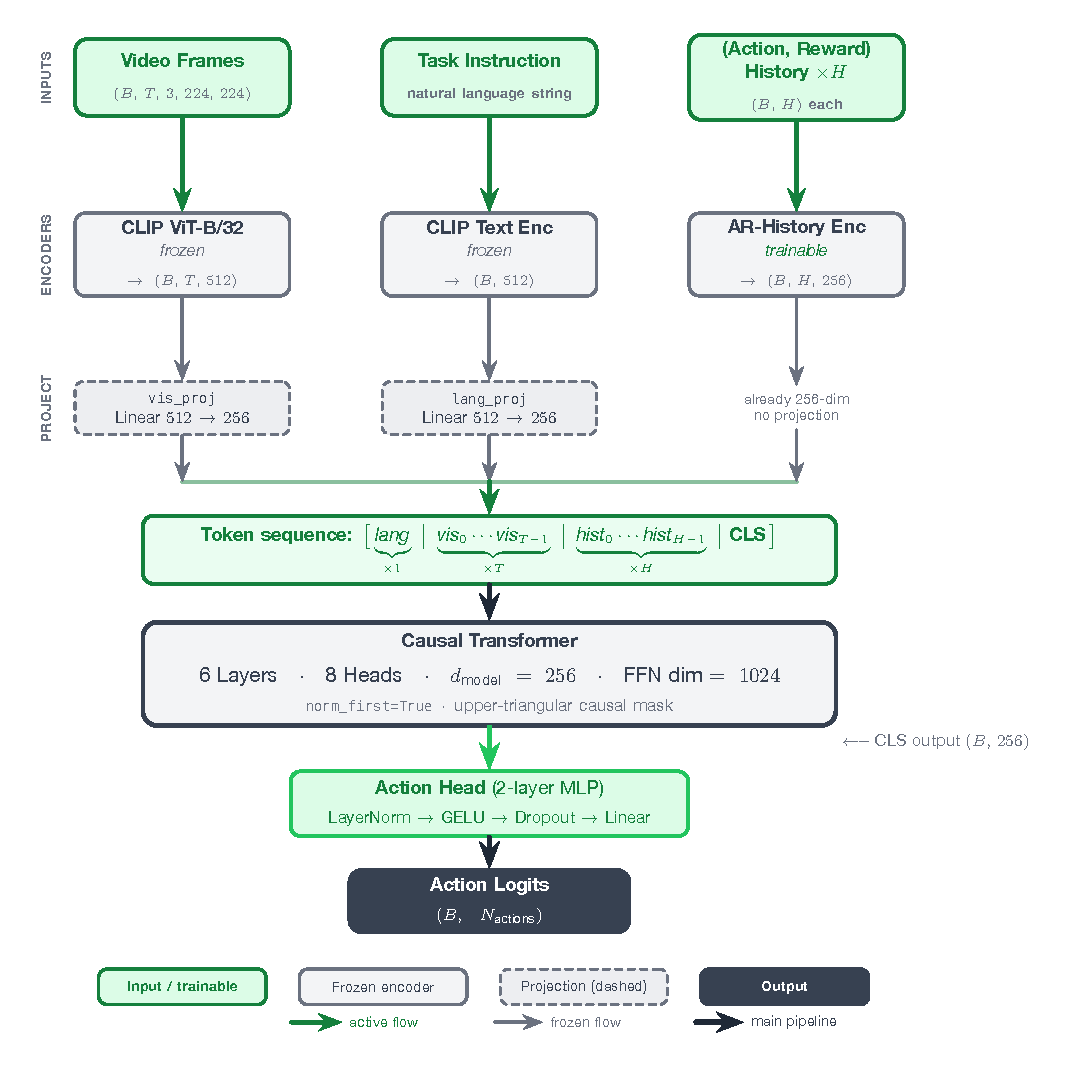
\includegraphics[width=\textwidth]{architecture_diagram.pdf}
\caption{%
  Full forward-pass architecture of \textbf{RLConditionedVLA}.
  Three input streams — video frames, a natural language instruction, and an
  (action, reward) history — are independently encoded, projected to a shared
  256-dim space, and assembled into a causal token sequence.
  The \textbf{CLS} token placed last attends to all preceding tokens
  (vision, language, history) via the upper-triangular causal mask, and its
  output is decoded by a two-layer MLP into discrete action logits.
  \textcolor{DarkGreen}{Green borders} = trainable or active-flow components;
  \textcolor{DimGray}{gray} = frozen CLIP encoders;
  \textbf{black} = main inference pipeline.
  See \texttt{architecture\_diagram.tex} for the standalone source.%
}
\label{fig:arch}
\end{figure}

\newpage

%% ============================================================================
\section{Introduction}
%% ============================================================================

\subsection{Motivation}

Modern robotics increasingly relies on large pretrained models to bridge the
gap between natural language instructions and physical actions.
Vision-Language-Action (VLA) models such as RT-2~\cite{brohan2023rt2} and
Octo~\cite{octo2024} have demonstrated that a model trained on internet-scale
image-text data can be fine-tuned to generate robot control signals.
However, these models treat each decision as a \emph{stateless} perception
problem: given the current image and instruction, predict the action.

This design ignores a fundamentally useful signal: \textbf{what the robot
just tried, and whether it worked}.
If a robot attempts to grasp an object and fails (reward $< 0$), a
history-conditioned policy can adapt its next action accordingly.
Without this signal, the policy has no mechanism to recover from repeated
mistakes.

\subsection{Problem Statement}

Given a task instruction $\ell$ (natural language) and the robot's observation
at time $t$ (video frame $s_t$), together with its recent interaction history
$\mathcal{H}_t = \{(a_{t-H},\,r_{t-H}),\ldots,(a_{t-1},\,r_{t-1})\}$,
predict the next action $a_t$ from a finite discrete action set
$\mathcal{A} = \{0, 1, \ldots, N-1\}$:

\[
  a_t = \pi_\theta\!\left(s_t,\;\ell,\;\mathcal{H}_t\right)
\]

where $\pi_\theta$ is the parameterised policy to be learned.

\subsection{Contributions}

\begin{itemize}[leftmargin=1.5em]
  \item A multimodal VLA architecture (\textbf{RLConditionedVLA}) that
        treats (action, reward) history as first-class input tokens,
        fused with vision and language via a causal Transformer.
  \item A two-phase training pipeline: behavioural cloning initialisation
        followed by online REINFORCE with a KL-divergence penalty to
        prevent forgetting.
  \item A modular codebase with a Gymnasium-compatible environment interface
        and a real-robot stub, supporting sim-to-real transfer.
  \item Identification and correction of a critical architectural bug
        (§\ref{sec:bug}) in which the CLS aggregation token was isolated from
        all other input tokens by the causal mask.
\end{itemize}

\subsection{Report Structure}

Section~\ref{sec:related} reviews related work.
Section~\ref{sec:arch} describes the overall architecture.
Section~\ref{sec:integration} explains step-by-step how the three models are
combined.
Section~\ref{sec:training} describes the training methodology.
Section~\ref{sec:impl} covers implementation details.
Section~\ref{sec:status} summarises the current project status.
Section~\ref{sec:discussion} discusses design choices.
Section~\ref{sec:future} outlines next steps.
Section~\ref{sec:conclusion} concludes.

\newpage

%% ============================================================================
\section{Related Work}
\label{sec:related}
%% ============================================================================

\subsection{Vision-Language Models}

CLIP~\cite{radford2021clip} introduced contrastive learning on 400M
image-text pairs, producing a shared embedding space where visual and textual
representations of the same concept are geometrically close.
The Vision Transformer (ViT)~\cite{dosovitskiy2021vit} underpins the CLIP
image encoder (ViT-B/32 in this work), partitioning images into 32$\times$32
pixel patches processed by self-attention layers.
We use CLIP's visual-semantic alignment as a frozen foundation, avoiding the
need for large task-specific vision datasets.

\subsection{Vision-Language-Action Models}

RT-2~\cite{brohan2023rt2} extends a 55-billion parameter vision-language
model to generate tokenised robot actions, achieving impressive zero-shot and
few-shot generalisation on manipulation tasks.
Octo~\cite{octo2024} provides a smaller (93M parameter), open-source
generalist policy designed specifically for fine-tuning on new tasks and
embodiments.
Both models treat inference as a one-shot perception problem without explicit
RL history conditioning, which is the primary gap this work addresses.

\subsection{Sequence Modelling for RL}

The Decision Transformer~\cite{chen2021decision} reframes offline RL as a
conditional sequence modelling problem: given a sequence of
(return-to-go, state, action) tokens, predict the next action.
This work adapts that idea to the online, multimodal setting: the history of
(action~index, reward) pairs is encoded as tokens and injected into the
Transformer's input sequence alongside vision and language tokens.

\subsection{RLHF and KL Regularisation}

Ouyang et~al.~\cite{ouyang2022rlhf} introduced KL-divergence penalties
against a reference model to prevent reinforcement learning from destroying
the knowledge acquired during supervised pretraining.
We apply the same strategy: the behavioural cloning checkpoint serves as a
frozen reference, and an explicit KL penalty keeps the RL policy from
diverging too far.

\newpage

%% ============================================================================
\section{System Architecture}
\label{sec:arch}
%% ============================================================================

\subsection{Overview}

\textbf{RLConditionedVLA} consists of four main components that are
composed in a strict pipeline:

\begin{enumerate}[leftmargin=1.5em]
  \item \textbf{CLIP Vision Encoder} — maps video frames to semantic embeddings.
  \item \textbf{CLIP Text Encoder} — maps the language instruction to a single
        goal embedding.
  \item \textbf{ActionRewardHistoryEncoder} — maps the discrete (action~index,
        scalar reward) history to a sequence of learned token embeddings.
  \item \textbf{Causal Fusion Transformer} — jointly reasons over all token
        types and produces the next discrete action via a classification head.
\end{enumerate}

\begin{lstlisting}[style=Diagram, caption={High-level data flow through RLConditionedVLA.}]
1 Video frames (B,T,3,224,224) --> CLIP ViT-B/32 --> vis_proj --> vis_tokens (B,T,256)
2 Language (B,77) --> CLIP text enc --> lang_proj --> lang_token (B,1,256)
3 (action,reward)xH --> AR-History-Enc --> hist_tokens (B,H,256)
4 |
5 [lang | vis_0..T-1 | hist_0..H-1 | CLS]
6 |
7 Causal Transformer (6 layers, 8 heads)
8 |
9 CLS output (B,256)
10 |
11 Action Head --> logits (B,N_actions)
\end{lstlisting}

\subsection{CLIP Backbone}

The CLIP ViT-B/32 model~\cite{radford2021clip} provides both the vision and
language encoders.
The image encoder splits each $224\times224$ frame into $7\times7 = 49$
non-overlapping patches of size $32\times32$ pixels.
Each patch is linearly projected to a 768-dimensional token, and 12 layers
of multi-head self-attention produce a 512-dimensional global image embedding
at the \texttt{[CLS]} position.

Frames are encoded independently (no temporal convolutions), allowing the
Transformer fusion stage to learn temporal relationships from positional
structure alone.
The text encoder applies the same transformer architecture to 77 BPE tokens,
producing a 512-dimensional sentence-level embedding at the \texttt{[EOS]}
position.

\subsection{Projection to Shared Space}

Both CLIP outputs are projected from 512 to 256 dimensions via learnable
linear layers (\texttt{vis\_proj} and \texttt{lang\_proj}).
The history encoder natively produces 256-dimensional tokens.
All three modalities therefore occupy the same embedding space before
entering the fusion Transformer.

\begin{notebox}
  The projection layers are trainable even when CLIP is frozen.
  They serve as a domain-adaptation interface, remapping CLIP's
  general-purpose embeddings towards the robot task distribution.
\end{notebox}

\subsection{ActionRewardHistoryEncoder}

For each of the $H$ history timesteps $i \in \{t-H,\ldots,t-1\}$:

\begin{align}
  \mathbf{a}_i &= \mathrm{Embedding}(a_i;\; W_a) \in \mathbb{R}^{256} \\
  \mathbf{r}_i &= \mathrm{Linear}(r_i;\; W_r) \in \mathbb{R}^{256} \\
  \mathbf{h}_i &= \mathrm{LayerNorm}\!\left(
      \mathrm{Linear}([\mathbf{a}_i\,\|\,\mathbf{r}_i]) + \mathbf{p}_i
    \right)
\end{align}

where $[\,\cdot\,\|\,\cdot\,]$ denotes concatenation,
$W_a \in \mathbb{R}^{(N+1)\times256}$ is the action embedding table
(the extra index $N$ is a learned ``no-action'' padding token for
cold-start),
$W_r \in \mathbb{R}^{1\times256}$ is the reward projection,
and $\mathbf{p}_i \in \mathbb{R}^{256}$ is a learned positional embedding
indexed by history slot $i$.

Stacking $H$ such vectors yields \texttt{hist\_tokens} $\in \mathbb{R}^{B \times H \times 256}$.

\subsection{Token Sequence and Causal Mask}

The complete input sequence to the Transformer is:

\[
  \mathbf{X} = [\,\mathbf{e}_\text{lang} \;\|\;
                   \mathbf{v}_{t-T}\,\cdots\,\mathbf{v}_{t-1} \;\|\;
                   \mathbf{h}_{t-H}\,\cdots\,\mathbf{h}_{t-1} \;\|\;
                   \mathbf{c}\,]
              \in \mathbb{R}^{(1+T+H+1) \times 256}
\]

where $\mathbf{c}$ is a learnable CLS token placed \textbf{last}.
An upper-triangular causal mask is applied, so position $i$ attends only to
positions $j \leq i$.
With CLS at the final position, it attends to every preceding token, making
it a full aggregation over language, visual, and history information.

\begin{lstlisting}[style=Diagram, caption={Causal attention mask for default config (T=3, H=4). Tick = attend, X = blocked.}]
           lang  v0   v1   v2   h0   h1   h2   h3   CLS
  lang  [   v     x    x    x    x    x    x    x    x  ]
  v0    [   v     v    x    x    x    x    x    x    x  ]
  v1    [   v     v    v    x    x    x    x    x    x  ]
  v2    [   v     v    v    v    x    x    x    x    x  ]
  h0    [   v     v    v    v    v    x    x    x    x  ]
  h1    [   v     v    v    v    v    v    x    x    x  ]
  h2    [   v     v    v    v    v    v    v    x    x  ]
  h3    [   v     v    v    v    v    v    v    v    x  ]
  CLS   [   v     v    v    v    v    v    v    v    v  ]  <- attends to everything
\end{lstlisting}

\subsection{Action Classification Head}

The CLS token output $\mathbf{c}' \in \mathbb{R}^{256}$ is passed through:

\[
  \hat{\mathbf{y}} = W_2\,\mathrm{GELU}\!\left(W_1\,\mathrm{LayerNorm}(\mathbf{c}')\right),
  \quad W_1 \in \mathbb{R}^{128\times256},\; W_2 \in \mathbb{R}^{N\times128}
\]

with dropout ($p=0.1$) after the GELU activation.
The output $\hat{\mathbf{y}} \in \mathbb{R}^{N}$ contains unnormalised action
logits.
At inference, the action is selected as $a_t = \arg\max_i \hat{y}_i$
(deterministic) or sampled from $\mathrm{softmax}(\hat{\mathbf{y}})$ (stochastic,
used during RL rollouts).

\subsection{Parameter Count}

\begin{table}[h]
\centering
\caption{Parameter breakdown of RLConditionedVLA (\texttt{freeze\_clip=True}).}
\begin{tabular}{L{6cm} r r}
\toprule
\textbf{Component} & \textbf{Parameters} & \textbf{Trainable} \\
\midrule
CLIP ViT-B/32 image encoder  & $\approx$86.2M & No  \\
CLIP text encoder             & $\approx$37.8M & No  \\
\texttt{vis\_proj}  Linear(512$\to$256) & 131,328  & Yes \\
\texttt{lang\_proj} Linear(512$\to$256) & 131,328  & Yes \\
ActionRewardHistoryEncoder    & $\approx$267K  & Yes \\
CLS token (learnable vector)  & 256            & Yes \\
Causal Transformer (6L, 8H)   & $\approx$3.2M  & Yes \\
Action head (2-layer MLP)     & $\approx$33K   & Yes \\
\midrule
\textbf{Total trainable}  & \textbf{$\approx$3.8M}  & \\
\textbf{Total (incl.\ frozen)} & \textbf{$\approx$128M} & \\
\bottomrule
\end{tabular}
\end{table}

\newpage

%% ============================================================================
\section{Model Integration — Step by Step}
\label{sec:integration}
%% ============================================================================

This section traces a single forward pass through \texttt{RLConditionedVLA.forward()}
with explicit tensor shapes and the reasoning behind each combination decision.

\subsection{The Core Problem: Incompatible Representations}

The three input streams cannot be directly combined because they live in
different mathematical spaces:

\begin{table}[h]
\centering
\caption{Raw input representations before encoding.}
\begin{tabular}{L{3.2cm} L{4.5cm} L{5cm}}
\toprule
\textbf{Modality} & \textbf{Raw format} & \textbf{Problem} \\
\midrule
Video frames      & Pixel tensors \newline$(B,T,3,224,224)$, uint8
                  & High-dimensional, spatial; no semantic structure \\
Language          & Integer token IDs \newline$(B,77)$, int64
                  & Symbolic, discrete; no overlap with pixel space \\
Action/reward history
                  & Mixed: int indices + float scalars, $(B,H)$ each
                  & Heterogeneous types; need token-like representation \\
\bottomrule
\end{tabular}
\end{table}

The solution is a four-step pipeline:
\begin{enumerate}[label=\textbf{\Roman*.}, leftmargin=2em]
  \item \textbf{Encode}: raw inputs $\rightarrow$ per-modality embeddings
  \item \textbf{Project}: per-modality embeddings $\rightarrow$ $\mathbb{R}^{256}$
  \item \textbf{Assemble}: $\mathbb{R}^{256}$ $\rightarrow$ token sequence
  \item \textbf{Fuse}: token sequence $\rightarrow$ action logits
\end{enumerate}

\subsection{Step 1 — Encode Vision with CLIP}
\label{sec:step1}

\textbf{Code:} \texttt{RLConditionedVLA.encode\_frames()} (line~117)

Frames are flattened from $(B,T,C,H,W)$ to $(B{\cdot}T,C,H,W)$ and
processed independently by the CLIP ViT-B/32 encoder.
Each frame is divided into 49 patches; self-attention across the 49 patch
tokens (plus one internal CLS token) produces a 512-dim global embedding.
The $(B{\cdot}T,512)$ output is reshaped to $(B,T,512)$ and projected
to $(B,T,256)$ by \texttt{vis\_proj}.

\textbf{Why encode each frame independently?}
The fusion Transformer handles temporal relationships across frame tokens.
Encoding frames independently keeps the CLIP encoder unchanged and avoids
the need for temporally-aware fine-tuning of the vision backbone.

\textbf{Why freeze CLIP?}
CLIP's 400M-pair pretraining produces visual embeddings where "red cube" and
an image of a red cube are geometrically close.
Unfreezing during early training with limited robot data would destroy this
alignment faster than it could be re-learned.

\subsection{Step 2 — Encode Language with CLIP}
\label{sec:step2}

\textbf{Code:} \texttt{RLConditionedVLA.encode\_language()} (line~129)

The CLIP tokeniser maps the instruction string to 77 BPE token IDs.
The CLIP text encoder applies 12 transformer layers to these tokens,
and the embedding at the \texttt{[EOS]} position captures the full
sentence meaning as a 512-dim vector.
This is projected to $(B,1,256)$ by \texttt{lang\_proj}, becoming a
\emph{single token} in the fusion sequence.

\textbf{Why CLIP and not BERT or T5?}
CLIP's text encoder was trained \emph{jointly} with its image encoder.
The sentence ``pick up the red cube'' has an embedding close to an image of
a red cube being picked up — an alignment that BERT and T5 do not possess.
Using CLIP for both modalities means the two encoders already ``speak the
same language'' before fusion begins.

\textbf{Why one token for the entire instruction?}
The instruction functions as a global goal context, not a word-level signal.
A single token at the head of the sequence allows all subsequent visual and
history tokens to attend leftward and incorporate the goal during their own
update steps, without inflating the sequence length.

\subsection{Step 3 — Encode (Action, Reward) History}
\label{sec:step3}

\textbf{Code:} \texttt{ActionRewardHistoryEncoder.forward()} (line~41)

The action index and scalar reward for each of the $H$ previous timesteps
are encoded separately and then fused:

\begin{itemize}[leftmargin=1.5em]
  \item \textbf{Action} (discrete int): passed through a learnable embedding
        table $W_a \in \mathbb{R}^{(N+1)\times256}$.
        An embedding table is used because action indices are categorical —
        index 3 does not mean ``three times more'' than index 1.
  \item \textbf{Reward} (continuous float): projected by
        $W_r \in \mathbb{R}^{1\times256}$, allowing the model to learn
        which magnitude ranges are significant.
  \item \textbf{Fusion}: the two 256-dim vectors are concatenated and
        projected back to 256-dim, producing a single token per timestep
        where the reward \emph{modifies} the meaning of the action.
  \item \textbf{Positional encoding}: a learned embedding $\mathbf{p}_i$
        per history slot tells the Transformer which step is oldest and which
        is newest.
\end{itemize}

\textbf{Cold-start padding:} at the beginning of an episode the robot has
no history.
Missing slots are filled with action index $N$ (a dedicated ``no-action''
embedding, not zero) and reward $0.0$.

\subsection{Step 4 — Project to a Shared 256-dim Space}
\label{sec:step4}

\begin{table}[h]
\centering
\caption{Dimension alignment before Transformer fusion.}
\begin{tabular}{L{4cm} C{3cm} C{2cm} C{3cm}}
\toprule
\textbf{Modality} & \textbf{Native dim} & \textbf{Projection} & \textbf{Output dim} \\
\midrule
CLIP vision      & 512 & \texttt{vis\_proj}  & 256 \\
CLIP language    & 512 & \texttt{lang\_proj} & 256 \\
History encoder  & 256 & (none)              & 256 \\
CLS token        & 256 & (parameter)         & 256 \\
\bottomrule
\end{tabular}
\end{table}

The 256-dim fusion space was chosen over CLIP's native 512 to halve the
Transformer parameter count and memory footprint while remaining large enough
for cross-modal reasoning across three modalities.

\subsection{Step 5 — Assemble the Token Sequence}
\label{sec:step5}

\textbf{Code:} \texttt{RLConditionedVLA.forward()} (line~161)

\begin{lstlisting}[style=Python, caption={Token sequence assembly (forward pass).}]
sequence = torch.cat(
    [lang_tokens_,   # (B, 1, 256)
     vis_tokens,     # (B, T, 256)
     hist_tokens,    # (B, H, 256)
     cls],           # (B, 1, 256)  <-- LAST
    dim=1
)   # shape: (B, 1+T+H+1, 256)  =  (B, 9, 256) with defaults T=3, H=4
\end{lstlisting}

The ordering is deliberate:

\begin{table}[h]
\centering
\caption{Rationale for token ordering in the sequence.}
\begin{tabular}{L{2.5cm} L{9cm}}
\toprule
\textbf{Position} & \textbf{Rationale} \\
\midrule
Language first & All later tokens attend leftward and see the goal context,
                 enabling instruction-conditioned visual attention. \\
Vision next     & Older frames before newer frames; the newest frame can
                 attend to the full frame history. \\
History last (before CLS)
                & History tokens can attend to both the instruction and the
                 visual context when updating their representations. \\
CLS at end      & With a causal mask, the last position attends to all
                 preceding tokens.
                 See §\ref{sec:bug} for the critical bug this ordering fixes. \\
\bottomrule
\end{tabular}
\end{table}

\subsection{Step 6 — Fuse with a Causal Transformer}
\label{sec:step6}

\textbf{Code:} \texttt{RLConditionedVLA.forward()} (line~165)

A \texttt{nn.TransformerEncoder} with 6 layers, 8 attention heads, and
FFN dimension 1024 ($= 4 \times 256$, the standard 4$\times$ expansion
from~\cite{vaswani2017attention}) processes the token sequence with a
causal mask.

Each layer computes:
\[
  \mathbf{X}^{(\ell+1)} = \mathrm{LayerNorm}\!\left(
    \mathbf{X}^{(\ell)} + \mathrm{MHA}\!\left(\mathbf{X}^{(\ell)},\,\mathbf{M}\right)
    + \mathrm{FFN}\!\left(\cdot\right)
  \right)
\]
where $\mathbf{M}$ is the upper-triangular boolean mask and pre-LayerNorm
ordering (\texttt{norm\_first=True}) follows modern practice (GPT-2, LLaMA)
for improved training stability.

After 6 layers, the CLS token at the last position has attended to all
9 tokens in the sequence.
The model has learned task-specific attention patterns, for example:
which visual tokens to focus on given a specific instruction, and how
the reward history should modify the interpretation of the visual scene.

\textbf{Why self-attention over the joint sequence rather than cross-attention?}
Cross-attention would require designating one modality as the ``query'' and
the others as ``keys/values'' — an arbitrary choice.
Joint self-attention lets every token attend to every other modality
symmetrically, with the mask imposing only temporal ordering.

\subsection{Step 7 — Read Out and Classify}
\label{sec:step7}

\textbf{Code:} \texttt{RLConditionedVLA.forward()} (line~170)

\begin{lstlisting}[style=Python, caption={CLS read-out and action classification.}]
cls_out = out[:, -1, :]          # (B, 256) -- last token = CLS
return self.action_head(cls_out) # (B, num_actions)
\end{lstlisting}

The two-layer action head (with LayerNorm, GELU, and Dropout) maps the
256-dim CLS representation to $N$-dimensional logits.
A two-layer MLP is used rather than a single linear layer because the CLS
token contains a mixed multimodal representation; the hidden layer and
nonlinearity allow the model to disentangle modality-specific information
before the final classification boundary.

\subsection{Why Not a Simpler Fusion Strategy?}
\label{sec:whynot}

\begin{table}[h]
\centering
\caption{Alternative fusion strategies considered and rejected.}
\begin{tabular}{L{4.5cm} L{8cm}}
\toprule
\textbf{Alternative} & \textbf{Reason for rejection} \\
\midrule
Concatenate + single MLP &
  Fixed fusion weights; cannot learn ``attend to red tokens when instruction
  says red''. All modalities mixed equally. \\
Late fusion (per-modality MLP, summed) &
  No cross-modal interaction before the decision.
  Cannot correlate ``bad reward'' with ``what the scene looked like''. \\
Cross-attention (history queries vision+lang) &
  Arbitrarily designates history as primary modality.
  Joint self-attention is strictly more flexible. \\
RNN over history &
  Implicit memory; gradients vanish; cannot inspect which past steps
  the model uses via attention weights. \\
Bidirectional transformer (no causal mask) &
  Loses temporal ordering inductive bias.
  Planned as ablation~A6. \\
\bottomrule
\end{tabular}
\end{table}

\subsection{Bug Found and Fixed: CLS Token Position}
\label{sec:bug}

\begin{bugbox}
\textbf{Discovered:} 2026-03-04 \hfill \textbf{Severity: Critical}

\textbf{Original code (incorrect):}
\begin{lstlisting}[style=Python, numbers=none]
sequence = torch.cat([cls, lang_tokens_, vis_tokens, hist_tokens], dim=1)
cls_out  = out[:, 0, :]   # reading from position 0
\end{lstlisting}

With CLS at position~0 and a causal mask, position~$i$ can only attend to
positions~$j \leq i$.
CLS at position~0 can only ever attend to itself — across \emph{all} 6
Transformer layers.
After $L$ layers: $\mathbf{c}^{(L)} = f^L(\mathbf{c}^{(0)})$, a function
only of the initial CLS parameter.
The action head therefore received zero information from vision, language,
or history. The entire CLIP encoding was ignored.

\textbf{Fix (correct):}
\begin{lstlisting}[style=Python, numbers=none]
sequence = torch.cat([lang_tokens_, vis_tokens, hist_tokens, cls], dim=1)
cls_out  = out[:, -1, :]  # reading from the last position
\end{lstlisting}

At the last position, the causal mask allows CLS to attend to all preceding
tokens across all layers, which is the intended aggregation behaviour.

\textbf{Files fixed:} \texttt{models/vla\_model.py} (lines 157, 166) and
\texttt{training/rl\_trainer.py} (lines 217, 223).
\end{bugbox}

\newpage

%% ============================================================================
\section{Training Methodology}
\label{sec:training}
%% ============================================================================

Training proceeds in two sequential phases.
Phase~1 provides a stable, demonstration-grounded initialisation.
Phase~2 refines the policy through environment interaction.

\subsection{Phase 1 — Behavioural Cloning (Supervised Fine-Tuning)}

Given a dataset $\mathcal{D} = \{(\mathbf{s}_t, \ell, \mathcal{H}_t,
a_t^*)\}$ of expert transitions, the model is trained to imitate the expert
action $a_t^*$ via cross-entropy loss with label smoothing~$\epsilon$:

\[
  \mathcal{L}_\text{BC} = -\sum_{a=0}^{N-1}
    \tilde{y}_a \log \hat{y}_a,
  \quad
  \tilde{y}_a = (1-\epsilon)\,\mathbf{1}[a = a_t^*] + \frac{\epsilon}{N}
\]

Label smoothing ($\epsilon = 0.05$) regularises against overconfident
predictions, which is important when expert demonstrations contain
ambiguous or sub-optimal actions.

\begin{table}[h]
\centering
\caption{Behavioural cloning hyperparameters.}
\begin{tabular}{L{5cm} L{3cm} L{5cm}}
\toprule
\textbf{Hyperparameter} & \textbf{Value} & \textbf{Rationale} \\
\midrule
Loss                & Cross-entropy   & Standard for discrete classification \\
Label smoothing $\epsilon$ & 0.05    & Prevents overconfidence on noisy demos \\
Optimiser           & AdamW           & Decoupled weight decay \\
Learning rate       & $3{\times}10^{-4}$ & Standard for Transformer fine-tuning \\
LR schedule         & Cosine $\to 10^{-6}$ & Smooth decay avoids late-stage oscillation \\
Gradient clip       & 1.0             & Stabilises early training \\
Batch size          & 32              & Fit in memory; stable gradient estimates \\
Epochs              & 50              & Adjust based on dataset size \\
Validation split    & 10\%            & Early stopping criterion \\
\bottomrule
\end{tabular}
\end{table}

\subsection{Phase 2 — Online RL Fine-Tuning (REINFORCE + Baseline)}

Starting from the Phase~1 checkpoint, the policy is refined through online
interaction using the REINFORCE algorithm~\cite{williams1992reinforce} with
a learned value baseline.

\textbf{Rollout collection:} for each update step, $K=4$ episodes are
collected by running the stochastic policy ($\pi(a|s) = \mathrm{softmax}(\hat{\mathbf{y}})$)
in the environment.

\textbf{Return computation:} discounted returns are computed at each step:
\[
  G_t = \sum_{k=0}^{T-t} \gamma^k r_{t+k}, \quad \gamma = 0.99
\]
Returns are normalised (zero mean, unit variance) within each batch to
reduce gradient variance.

\textbf{Composite loss:}
\[
  \mathcal{L}_\text{RL} =
    \underbrace{-\mathbb{E}\!\left[\log\pi(a_t|s_t)\cdot(G_t - V(s_t))\right]}_{\text{policy loss (REINFORCE)}}
    + \underbrace{0.5\,\mathbb{E}\!\left[(V(s_t)-G_t)^2\right]}_{\text{value baseline loss}}
    - \underbrace{0.01\,\mathcal{H}[\pi]}_{\text{entropy bonus}}
    + \underbrace{0.1\,D_\text{KL}(\pi \,\|\, \pi_\text{BC})}_{\text{KL penalty}}
\]

\begin{table}[h]
\centering
\caption{RL loss component rationale.}
\begin{tabular}{L{3.5cm} L{2cm} L{7cm}}
\toprule
\textbf{Term} & \textbf{Coef.} & \textbf{Purpose} \\
\midrule
Policy loss (REINFORCE) & 1.0 & Increase probability of high-return actions \\
Value baseline loss     & 0.5 & Reduce gradient variance via advantage \\
Entropy bonus           & 0.01 & Prevent premature collapse to a single action \\
KL divergence penalty   & 0.1  & Prevent catastrophic forgetting of BC policy \\
\bottomrule
\end{tabular}
\end{table}

The KL penalty uses a frozen copy of the Phase~1 checkpoint as the reference
distribution $\pi_\text{BC}$, following the RLHF approach of
Ouyang et~al.~\cite{ouyang2022rlhf}.

\subsection{Evaluation Protocol}

After each training phase, the policy is evaluated over 50 deterministic
($\arg\max$) episodes.
Reported metrics: mean episode return~$\pm$~std, mean episode length, and
success rate (episodes where cumulative return $\geq$ threshold).

\newpage

%% ============================================================================
\section{Implementation Details}
\label{sec:impl}
%% ============================================================================

\subsection{File Structure}

\begin{lstlisting}[style=Diagram, caption={Project directory layout.}]
VLA-Robot-Learning/
  models/
    vla_model.py             -- RLConditionedVLA, ActionRewardHistoryEncoder
  training/
    sft_trainer.py           -- Phase 1: behavioural cloning
    rl_trainer.py            -- Phase 2: REINFORCE + value baseline + KL
  data/
    trajectory_dataset.py    -- TrajectoryDataset, episode I/O utilities
  envs/
    sim_env.py               -- SimEnv (Gym wrapper), RealEnv (robot stub)
  evaluation/
    evaluate.py              -- N-episode rollout and metrics
  configs/
    config.yaml              -- all hyperparameters
  REPORT.tex                 -- this document
  REPORT.md                  -- living notes (compiled to PDF via generate_report.py)
  generate_report.py         -- pandoc/xelatex PDF builder + watch mode
  references.bib             -- BibTeX entries
\end{lstlisting}

\subsection{Episode Data Format}

Each episode is stored as a Python dictionary:

\begin{lstlisting}[style=Python, caption={Episode dictionary format.}]
episode = {
    "frames":      np.ndarray,  # (T_ep, H, W, 3) uint8
    "instruction": str,          # natural-language task goal
    "actions":     np.ndarray,  # (T_ep,) int64 -- discrete indices
    "rewards":     np.ndarray,  # (T_ep,) float32
}
\end{lstlisting}

Episodes are stored as a \texttt{.pkl} file (list of dicts).
If no real data is available, \texttt{make\_random\_episodes()} generates
synthetic episodes for end-to-end pipeline testing.

\subsection{Environment Interface}

All environments implement the \texttt{BaseEnv} interface:

\begin{lstlisting}[style=Python, caption={BaseEnv interface.}]
class BaseEnv:
    def reset(self) -> dict:          # {"frame": ndarray, "instruction": str}
        ...
    def step(self, action: int):      # -> (obs, reward, done, info)
        ...
\end{lstlisting}

The \texttt{SimEnv} class wraps any Gymnasium environment with
\texttt{render\_mode="rgb\_array"}.
The \texttt{RealEnv} stub is ready to be wired to a physical robot SDK
(camera capture and joint/gripper control).

\subsection{Running the Pipeline}

\begin{lstlisting}[style=Bash, caption={Training and evaluation commands.}]
# Phase 1: Behavioural Cloning
python -m training.sft_trainer --config configs/config.yaml

# Phase 2: RL Fine-Tuning (requires best_sft.pt from Phase 1)
python -m training.rl_trainer --config configs/config.yaml

# Evaluation (deterministic)
python -m evaluation.evaluate \
    --config configs/config.yaml \
    --checkpoint checkpoints/rl/best_rl.pt \
    --episodes 50

# Regenerate this PDF
python generate_report.py --tex
\end{lstlisting}

\newpage

%% ============================================================================
\section{Current Project Status}
\label{sec:status}
%% ============================================================================

\begin{table}[h]
\centering
\caption{Component completion status.}
\begin{tabular}{L{6cm} C{2.5cm} L{4cm}}
\toprule
\textbf{Component} & \textbf{Status} & \textbf{File} \\
\midrule
Core model architecture    & \textcolor{SuccessGreen}{\textbf{Done}} & \texttt{models/vla\_model.py} \\
History encoder            & \textcolor{SuccessGreen}{\textbf{Done}} & \texttt{models/vla\_model.py} \\
CLS bug fix                & \textcolor{SuccessGreen}{\textbf{Done}} & both model files \\
Trajectory dataset         & \textcolor{SuccessGreen}{\textbf{Done}} & \texttt{data/trajectory\_dataset.py} \\
Behavioural cloning trainer& \textcolor{SuccessGreen}{\textbf{Done}} & \texttt{training/sft\_trainer.py} \\
RL fine-tuning trainer     & \textcolor{SuccessGreen}{\textbf{Done}} & \texttt{training/rl\_trainer.py} \\
Value head                 & \textcolor{SuccessGreen}{\textbf{Done}} & \texttt{training/rl\_trainer.py} \\
KL penalty                 & \textcolor{SuccessGreen}{\textbf{Done}} & \texttt{training/rl\_trainer.py} \\
Gym environment wrapper    & \textcolor{SuccessGreen}{\textbf{Done}} & \texttt{envs/sim\_env.py} \\
Real robot interface stub  & \textcolor{SuccessGreen}{\textbf{Done}} & \texttt{envs/sim\_env.py} \\
Evaluation script          & \textcolor{SuccessGreen}{\textbf{Done}} & \texttt{evaluation/evaluate.py} \\
Config file                & \textcolor{SuccessGreen}{\textbf{Done}} & \texttt{configs/config.yaml} \\
\midrule
Real demonstration data    & \textcolor{AlertRed}{\textbf{Pending}} & — \\
Gym environment selection  & \textcolor{AlertRed}{\textbf{Pending}} & — \\
SFT training run           & \textcolor{AlertRed}{\textbf{Pending}} & — \\
RL training run            & \textcolor{AlertRed}{\textbf{Pending}} & — \\
TensorBoard logging        & \textcolor{AlertRed}{\textbf{Pending}} & — \\
PPO upgrade                & \textcolor{AlertRed}{\textbf{Pending}} & — \\
\bottomrule
\end{tabular}
\end{table}

\subsection{Experiment Log}

\begin{table}[h]
\centering
\caption{Experiment results (to be filled in as experiments are run).}
\begin{tabular}{L{2cm} L{2cm} L{2.5cm} C{1.5cm} C{3cm} L{3cm}}
\toprule
\textbf{Date} & \textbf{Phase} & \textbf{Environment} & \textbf{Epochs} & \textbf{Val Acc / Return} & \textbf{Notes} \\
\midrule
— & — & — & — & — & Pending \\
\bottomrule
\end{tabular}
\end{table}

\newpage

%% ============================================================================
\section{Discussion}
\label{sec:discussion}
%% ============================================================================

\subsection{Strengths of the Proposed Architecture}

\textbf{Explicit RL memory.}
By encoding (action, reward) history as explicit tokens, the model's
``reasoning'' over past experience is inspectable: attention weights between
the CLS token and specific history tokens reveal which previous steps
the model considers most relevant to the current decision.
This is impossible with RNN-based memory.

\textbf{CLIP alignment.}
Using CLIP for both vision and language encoders means the embeddings arrive
in a pre-aligned space.
The fusion Transformer does not need to learn to bridge the visual-linguistic
modality gap from scratch — it only needs to learn task-specific routing.

\textbf{Modular design.}
The three encoders are decoupled.
Replacing the CLIP vision backbone with a domain-specific encoder (e.g.,
a depth-image encoder for indoor navigation) requires only changing
\texttt{encode\_frames()} and \texttt{vis\_proj}.

\subsection{Limitations}

\textbf{Global visual token only.}
CLIP's \texttt{[CLS]} output is a \emph{global} image embedding — it has no
spatial resolution.
Tasks requiring precise spatial reasoning (e.g., grasping a specific part of
an object) may benefit from using CLIP's per-patch tokens instead.

\textbf{Discrete actions only (current).}
Continuous control (joint angles, end-effector velocities) is not currently
supported.
Adding a regression head or tokenising continuous actions in the RT-2 style
is a planned extension.

\textbf{REINFORCE variance.}
REINFORCE has high gradient variance even with a baseline.
PPO~\cite{schulman2017ppo} provides a clipped surrogate objective that
is more stable for long episodes and sparse reward settings.

\subsection{Comparison with Related Models}

\begin{table}[h]
\centering
\caption{Comparison with related VLA models.}
\begin{tabular}{L{3cm} C{2.2cm} C{2cm} C{2cm} C{2.5cm} C{2cm}}
\toprule
\textbf{Model} & \textbf{Params} & \textbf{Action type} & \textbf{RL history} & \textbf{Open source} & \textbf{GPU req.} \\
\midrule
RT-2             & 55B  & Tokenised cont. & No  & No  & TPU \\
Octo             & 93M  & Continuous      & No  & Yes & A100 \\
\textbf{Ours}    & \textbf{3.8M trainable} & \textbf{Discrete} & \textbf{Yes} & \textbf{Yes} & \textbf{Consumer GPU} \\
\bottomrule
\end{tabular}
\end{table}

\newpage

%% ============================================================================
\section{Future Work \& Next Steps}
\label{sec:future}
%% ============================================================================

\subsection{Immediate (Phase A — Get Pipeline Running)}

\begin{enumerate}[leftmargin=1.5em]
  \item \textbf{Choose simulation environment.}
        Candidates: MiniGrid-Empty-5x5 (simplest discrete action space),
        FetchReach-v2 (realistic manipulation), FrankaKitchen-v1 (hardest).
  \item \textbf{Define action space.}
        Enumerate the exact $N$ discrete actions; update \texttt{config.yaml}.
  \item \textbf{Collect demonstration data.}
        Run a scripted or random policy in the chosen environment;
        save as \texttt{data/episodes.pkl}.
  \item \textbf{Run Phase~1 SFT} and verify validation accuracy is non-trivial.
  \item \textbf{Evaluate Phase~1 checkpoint} on 50 episodes; record results in
        Table~8.
\end{enumerate}

\subsection{Short-term (Phase B — RL Fine-Tuning)}

\begin{enumerate}[leftmargin=1.5em]
  \item Run Phase~2 RL; monitor mean return per epoch.
  \item Add TensorBoard logging to both trainers.
  \item Compare Phase~1 and Phase~2 checkpoints on the same evaluation set.
\end{enumerate}

\subsection{Medium-term (Phase C — Improve \& Ablate)}

\begin{table}[h]
\centering
\caption{Planned ablation studies.}
\begin{tabular}{C{0.8cm} L{3.5cm} L{5cm} L{4cm}}
\toprule
\textbf{\#} & \textbf{Ablation} & \textbf{Change} & \textbf{Expected outcome} \\
\midrule
A1 & No history        & \texttt{history\_len=0}               & Lower recovery performance \\
A2 & Action-only hist. & Remove reward from encoder            & Slightly worse \\
A3 & Unfreeze CLIP     & \texttt{freeze\_clip: false}          & Better with large data \\
A4 & PPO vs REINFORCE  & Replace \texttt{rl\_trainer} algorithm & More stable training \\
A5 & History length    & $H \in \{1,2,4,8\}$                  & Find optimal window \\
A6 & Bidirectional attn. & Remove causal mask                  & Marginal change \\
\bottomrule
\end{tabular}
\end{table}

\subsection{Long-term (Phase D — Sim-to-Real)}

\begin{enumerate}[leftmargin=1.5em]
  \item Enable domain randomisation (\texttt{env.domain\_randomization: true});
        tune observation noise.
  \item Implement \texttt{RealEnv} with physical camera and robot SDK.
  \item Evaluate on real robot; report success rate.
\end{enumerate}

\newpage

%% ============================================================================
\section{Conclusion}
\label{sec:conclusion}
%% ============================================================================

This report documents the design, implementation, and current status of
\textbf{RLConditionedVLA}, a Vision-Language-Action model that conditions
robot action prediction on an explicit history of (action, reward) pairs.

The key architectural contribution is the treatment of RL feedback as
first-class input tokens, fused with CLIP-encoded vision and language
features via a six-layer causal Transformer.
This explicit, token-based memory is inspectable (via attention weights),
cold-start-robust (via dedicated padding tokens), and naturally extensible
to longer histories or multi-step action generation.

A critical bug — in which the CLS aggregation token was isolated from all
other tokens by the causal mask — was identified and corrected during
architectural analysis, underscoring the importance of carefully reasoning
about the interaction between positional ordering and attention masking.

The full training pipeline (behavioural cloning followed by REINFORCE with
KL regularisation) and evaluation framework are implemented and ready for
execution once demonstration data and a target environment are selected.

\bigskip
\noindent\textbf{Next action item:} select a Gymnasium environment and collect
the first batch of demonstration episodes (Phase A, Step~1).

%% ── References ───────────────────────────────────────────────────────────────
\newpage
\bibliographystyle{ieeetr}
\bibliography{references}

%% ── Appendix ─────────────────────────────────────────────────────────────────
\newpage
\appendix

\section{Issues \& Fixes Log}

\begin{table}[h]
\centering
\caption{All bugs and fixes recorded chronologically.}
\begin{tabular}{L{2cm} L{4.5cm} L{4.5cm} L{2cm}}
\toprule
\textbf{Date} & \textbf{Issue} & \textbf{Fix} & \textbf{File} \\
\midrule
2026-03-03 &
  \texttt{--highlight-style} deprecated in pandoc 3.9; LaTeX error from
  complex YAML \texttt{header-includes} &
  Removed \texttt{header-includes}; passed all styling as pandoc \texttt{-V}
  CLI variables &
  \texttt{generate\_report.py} \\[6pt]
2026-03-04 &
  CLS token at position 0 with causal mask is isolated — never attends to
  vision, language, or history tokens across any layer &
  Moved CLS to last position; read \texttt{out[:, -1, :]} &
  \texttt{models/vla\_model.py}, \texttt{training/rl\_trainer.py} \\
\bottomrule
\end{tabular}
\end{table}

\section{Change Log}

\begin{table}[h]
\centering
\caption{Project change log.}
\begin{tabular}{L{2.5cm} L{10.5cm}}
\toprule
\textbf{Date} & \textbf{Change} \\
\midrule
2026-03-03 &
  Project initialised. Full codebase scaffolded: model, SFT trainer,
  RL trainer, dataset, sim env, evaluation, config, PDF report generator. \\[4pt]
2026-03-04 &
  \texttt{REPORT.md} restructured with detailed architecture diagrams,
  token sequence layout, parameter count table, and prioritised next steps. \\[4pt]
2026-03-04 &
  \texttt{REPORT.tex} created: full academic-format \LaTeX{} report with
  title page, abstract, TOC, and all sections. \\[4pt]
2026-03-04 &
  Bug fixed: CLS token at position 0 isolated by causal mask.
  Moved to last position in \texttt{models/vla\_model.py} and
  \texttt{training/rl\_trainer.py}. \\
\bottomrule
\end{tabular}
\end{table}

\end{document}
